%% Conference version (condensed)
\documentclass[conference]{IEEEtran}

% *** PACKAGES ***
\usepackage{amsmath,amssymb,amsfonts}
\usepackage{graphicx}
\usepackage{booktabs}
\usepackage{multirow}
\usepackage{array}
\usepackage{adjustbox}
\usepackage[font=small,labelfont=bf]{caption}
\usepackage{cite}
\usepackage{url}
\usepackage{hyperref}
\usepackage{algorithm}
\usepackage{algpseudocode}
\usepackage{tikz}
\usetikzlibrary{arrows.meta,decorations.pathreplacing}

\hyphenation{op-tical net-works semi-conduc-tor}

\begin{document}

\title{LIV-TS: Evolutionary Architecture Search for Time Series Forecasting via Linear Input-Varying Systems}

\author{Anonymous Authors}

\maketitle

% ==================== ABSTRACT ====================
\begin{abstract}
Contemporary state-of-the-art time series forecasting models, including S-Mamba \cite{wang2024smamba} and iTransformer \cite{liu2024itransformer}, achieve strong performance but hardcode specific operator choices (Mamba recurrence, self-attention, or feedforward networks) for each architectural component.
This rigid assignment assumes a universal inductive bias that may not hold across diverse datasets and forecasting horizons.
We propose \textbf{LIV-TS}, a framework that casts time series forecasting architecture design as a multi-objective evolutionary search over \emph{Linear Input-Varying} (LIV) \cite{massaroli2024liv} operators.
LIV provides a unified parameterization of attention, state-space models (SSMs), gated convolutions, and feedforward networks under a single token-mixing matrix whose structure determines the operator family.
We instantiate LIV operators inside two established forecasting structures (S-Mamba and iTransformer) and apply NSGA-II \cite{deb2002nsga2} to jointly optimize forecasting accuracy and model compactness.
Additionally, we adapt the Think-in-Diffusion Autoregressive (TiDAR) \cite{tidar2024} training scheme for continuous-valued time series, enabling parallel draft prediction with optional autoregressive refinement.
Experiments on the ETT benchmark and Exchange-Rate dataset reveal that evolutionary search consistently discovers \emph{heterogeneous} operator mixtures that occupy Pareto-optimal operating points no homogeneous baseline can match: on ETTh1 at $H\!=\!96$, the best mixed genome achieves MSE 0.464 at 1.2M parameters, matching the accuracy of the all-FFN baseline (MSE 0.454, 3.2M parameters) within 2\% at less than 40\% of its parameter cost --- a trade-off unavailable to any single-operator configuration.
Our results demonstrate that operator-family selection is a critical yet underexplored axis of time series model design, and that evolutionary search over a unified LIV operator pool reliably identifies compact, accurate architectures whose structural biases transfer across temporally compatible datasets and support fast parallel inference.
\end{abstract}

\begin{IEEEkeywords}
Time series forecasting, neural architecture search, linear input-varying systems, state-space models, evolutionary optimization, NSGA-II, attention mechanisms, autoregressive refinement.
\end{IEEEkeywords}

% ==================== CHAPTERS ====================
\section{Introduction}
\label{sec:intro}

Multivariate time series forecasting is a cornerstone task in domains ranging from energy grid management and financial trading to climate science and traffic control \cite{wu2021autoformer,zhou2021informer}.
Accurate multi-step predictions over long horizons require models that can simultaneously capture local temporal patterns, long-range dependencies, and inter-variate correlations: three qualitatively different phenomena that may benefit from different computational inductive biases.

Recent architectures have tackled this challenge by specializing each architectural component for a fixed operator family.
iTransformer \cite{liu2024itransformer} treats each variate as a token and uses self-attention for cross-variate correlation alongside a feedforward network (FFN) for per-variate feature extraction;
S-Mamba \cite{wang2024smamba} applies bidirectional Mamba recurrence for variate correlation followed by an FFN for temporal refinement.
These designs encode strong prior beliefs: \emph{attention is best for cross-variate mixing} and \emph{Mamba recurrence is best for temporal modeling}.
While each assumption yields strong results on particular benchmarks, it is unclear whether any single operator family universally excels, or whether the optimal operator varies with dataset characteristics and forecast horizon.

The importance of this choice is illustrated by a concrete comparison.
On ETTh1 at horizon H\,=\,96 using the iTransformer structure, replacing self-attention with a 3-tap gated convolution (GConv-1) reduces test MSE from 0.476 to 0.467 while using 33\% fewer parameters.
Conversely, using Mamba SSM across all slots inflates parameter count to 17M and degrades MSE to 1.213.
These results suggest that the \emph{choice of operator family per slot} is a high-impact yet underexplored design dimension.
Manual search over all combinations is intractable: with eleven base operator classes, four slots per structure, and differential variants, the search space exceeds $10^{5}$ configurations per structure.
Automated neural architecture search (NAS) \cite{elsken2019neural,zoph2017neural} offers a principled alternative, but existing NAS methods for time series focus on hyperparameter tuning rather than operator-family selection.

To address this gap, we propose \textbf{LIV-TS}, a framework built on two components.
First, following the Linear Input-Varying (LIV) framework \cite{thomas2024star,massaroli2024liv}, we express all mixing operators (self-attention variants, state-space models, gated convolutions, and feedforward networks) as instances of a token-mixing matrix $T_{ij}(x)$ whose structural pattern determines the operator family:
\begin{itemize}
  \item \emph{LOW\_RANK}: $T = CB^\top / \sqrt{d}$, which recovers multi-head self-attention (SA-1 through SA-4);
  \item \emph{SEMI\_SEPARABLE}: $T_{ij} = C_i\!\prod_{k=j}^{i-1}\!A_k\,B_j$, which recovers SSMs including Mamba and Closed-form Continuous-time networks (CfC);
  \item \emph{TOEPLITZ}: $T_{ij} = C_i K_{i-j} B_j$, which recovers local and long-range input-dependent convolutions;
  \item \emph{DIAGONAL}: $T_{ij} = C_i B_i \delta_{ij}$, which recovers element-wise gating (SwiGLU FFN).
\end{itemize}
This unification lets us treat all operators as interchangeable genome entries.
Second, we encode each forecasting architecture as a genome of LIV class identifiers (one per operator slot) and run NSGA-II \cite{deb2002nsga2} to simultaneously minimize validation MSE and parameter count, with the Pareto frontier balancing accuracy against model compactness without requiring explicit weighting.
Additionally, we integrate the Think-in-Diffusion Autoregressive (TiDAR) training scheme \cite{tidar2024} into LIV-TS, enabling parallel draft prediction of all $H$ future steps in a single forward pass with optional autoregressive refinement, which is particularly valuable for long-horizon settings where sequential decoding is prohibitively slow.

The main contributions of this work are:
\begin{enumerate}
  \item \textbf{LIV-TS framework.}
    We formalize time series forecasting architecture search within the LIV operator algebra, providing a clean genome encoding compatible with two structural templates (S-Mamba-style and iTransformer-style) and an operator pool that spans attention, convolution, SSM, and Closed-form Continuous-time (CfC) \cite{hasani2022liquid} recurrence classes.

  \item \textbf{Multi-objective evolutionary search.}
    We demonstrate that NSGA-II discovers heterogeneous operator mixtures (combining convolution, attention, and SSM variants within a single model) that dominate any single-class baseline on the Pareto frontier of accuracy versus parameter count.

  \item \textbf{TiDAR adaptation for continuous time series.}
    We adapt TiDAR's joint autoregressive--diffusion loss to continuous-valued forecasting and show that the draft mode achieves an 80.8$\times$ wall-clock speedup over full autoregressive decoding with negligible accuracy loss.

  \item \textbf{Cross-dataset architecture transfer.}
    We show that genomes discovered on ETTh1 transfer to ETTh2 and Exchange-Rate, outperforming the all-SSM baseline by up to 63\% in test MSE without retraining, providing evidence that evolutionary search recovers structurally meaningful inductive biases.
\end{enumerate}

The remainder of this paper is organized as follows.
Section~\ref{sec:background} reviews existing time series forecasting architectures and related work on NAS and unified sequence operators.
Section~\ref{sec:prelim} introduces the technical foundations: the LIV operator algebra, CfC networks, NSGA-II, and TiDAR.
Section~\ref{sec:method} describes the LIV-TS genome encoding, structural templates, fitness evaluation, and TiDAR adaptation.
Section~\ref{sec:experiments} presents experiments on operator ablation, full architecture search, TiDAR speedup, and cross-dataset transfer.
Section~\ref{sec:discussion} analyzes when heterogeneous architectures outperform single-operator models and characterizes the discovered Pareto fronts.
Section~\ref{sec:conclusion} concludes and outlines future directions.
  % Introduction
\section{Background and Related Work}
\label{sec:background}

\subsection{Time Series Forecasting Architectures}

Multivariate long-sequence forecasting has evolved through several architectural paradigms.
Early Transformer-based models such as Informer \cite{zhou2021informer} and Autoformer \cite{wu2021autoformer} apply attention over the \emph{temporal} axis, treating each time-step as a token.
This yields $\mathcal{O}(L^2)$ complexity and conflates temporal modelling with cross-variate modelling, since each token mixes all $C$ variates at a single time-step.

A decisive shift came with the observation that \emph{inverting} the token definition---making each variate a token---decouples variate correlation from temporal structure and reduces attention cost to $\mathcal{O}(C^2)$ when $C \ll L$.
iTransformer \cite{liu2024itransformer} operationalises this by embedding each variate's full $L$-step history into a single $D$-dimensional token, applying self-attention across the $C$ variate tokens for cross-variate mixing, and a per-variate FFN for feature transformation.
S-Mamba \cite{wang2024smamba} adopts the same variate-token layout but replaces the single backbone with a two-stage pipeline: a bidirectional Mamba block for variate correlation followed by an FFN block for temporal refinement.
DLinear \cite{zeng2023dlinear} challenges the necessity of complex operators entirely, showing that a simple decomposition plus linear projection is surprisingly competitive, motivating investigation into whether operator complexity should be matched to each task.
PatchTST \cite{nie2023patchtst} and TimesNet \cite{wu2023timesnet} explore patched temporal tokens and 2D convolutional representations respectively, further diversifying the design space.

Across these models a common pattern emerges: each design \emph{commits} to a specific operator for each architectural slot without empirical justification for that choice.
This motivates an operator-agnostic search over a unified operator family.

\subsection{Linear Input-Varying (LIV) Operators}

The LIV framework \cite{thomas2024star,massaroli2024liv} provides a unified algebraic view of sequence mixing operators.
Its central insight is to replace the \emph{fixed} weight matrix of a standard linear layer with a weight that is \emph{assembled from the input itself}.

In a standard linear layer the output is $Y = Wx$, where $W$ is a learned parameter independent of $x$.
In a LIV block, four learned linear projections of $x$ first produce feature vectors $B$, $C$, $S$, $V$:
\begin{equation}
  B = W_B x, \quad C = W_C x, \quad S = f_S(x), \quad V = W_V x,
  \label{eq:featurizer}
\end{equation}
where $W_B, W_C, W_V$ are plain \texttt{nn.Linear} layers (single matrix multiplies) and $f_S$ is either a linear layer with a learned bias or, for the input-dependent convolution case, a small two-layer MLP.
These are called the \emph{featurizer}.

The $L \times L$ token-mixing matrix $T$ is then \emph{assembled algebraically} from $B$, $C$, and $S$ — the four projections have distinct roles:

\begin{itemize}
  \item $\mathbf{b}_j$ and $\mathbf{c}_i$ (rows of $B$ and $C$) \textbf{dot-product to produce the scalar gate strength} of each entry $T_{ij}$.
        Their inner product $\langle\mathbf{c}_i, \mathbf{b}_j\rangle$ measures how strongly position $i$ should attend to position $j$.
  \item $S$ \textbf{provides the structural scalar} $M_{ij}$ that further modulates the gate strength: it encodes the \emph{pattern} (a decay factor for SSMs, a kernel value for convolutions, the constant 1 for attention, or absent for the diagonal case).
  \item $V$ \textbf{carries the payload}: it never enters the construction of $T$ at all.
        Once $T$ is assembled, the token-mixed output is obtained by $T \cdot V$, which routes the actual feature content.
\end{itemize}

Concretely, each entry of $T$ is:
\begin{equation}
  T_{ij} = \underbrace{\langle\mathbf{c}_i,\, \mathbf{s}_{ij} \odot \mathbf{b}_j\rangle}_{\text{gate strength modulated by structure}},
  \label{eq:tij}
\end{equation}
where $\mathbf{s}_{ij} \in \mathbb{R}^d$ is the \emph{structural modulator} derived from $S$ — for LOW\_RANK it is the all-ones vector; for SEMI\_SEPARABLE it is the element-wise cumulative product $\prod_{k=j}^{i-1}\mathbf{a}_k$ of transition vectors from $S$; for TOEPLITZ it is a scalar $K_{i-j}$ broadcast from $S$.

The full LIV forward pass is:
\begin{align}
  \mathrm{mixed}_i &= \sum_j T_{ij} \cdot \mathbf{v}_j, \quad \mathbf{v}_j = \text{$j$-th row of } V,
  \label{eq:token_mix} \\
  Y_i &= W \cdot \mathrm{mixed}_i,
  \label{eq:channel_mix}
\end{align}
where $W$ is a \emph{static} \texttt{nn.Parameter} — a fixed learned matrix independent of $x$.
The net computation is: (1) project $x$ to $B, C, S, V$ via linear layers; (2) assemble $T$ from $B, C, S$ algebraically; (3) mix content with $\mathrm{mixed} = T \cdot V$; (4) project with fixed $W$.

\subsubsection{Token Mixing Families}

Four choices of how $S$ constructs $\mathbf{s}_{ij}$ span the space of practical sequence operators.

\textbf{LOW\_RANK} — $\mathbf{s}_{ij} = \mathbf{1}/\sqrt{d}$ (constant, S unused):
\begin{equation}
  T_{ij} = \langle\mathbf{c}_i,\, \mathbf{b}_j\rangle / \sqrt{d}, \qquad T = CB^\top / \sqrt{d}.
\end{equation}
Every pair $(i,j)$ interacts with equal structural weight; row-wise softmax recovers multi-head attention \cite{vaswani2017attention}.
Cost $\mathcal{O}(L^2 d)$; full bidirectional context.

\textbf{SEMI\_SEPARABLE} — $\mathbf{s}_{ij} = \prod_{k=j}^{i-1}\mathbf{a}_k$ (S gives forget gate $\mathbf{a}_k$ per step):
\begin{equation}
  T_{ij} = \left\langle\mathbf{c}_i,\; \left(\prod_{k=j}^{i-1}\mathbf{a}_k\right) \odot \mathbf{b}_j\right\rangle \;\; (j \le i), \quad T_{ij} = 0 \;\; (j > i),
\end{equation}
where $\mathbf{a}_k \in (0,1)^d$ is the per-step forget gate (the $k$-th row of $S$), and $\mathbf{b}_j$ is the input contribution at position $j$.
The structural product $\prod_{k=j}^{i-1}\mathbf{a}_k$ decays the contribution of position $j$ exponentially as it propagates forward to position $i$; it is computed once via \texttt{torch.cumprod} and shared across all pairs without any per-element network call.
In this work we use CfC \cite{hasani2021cfc} as the sole SEMI\_SEPARABLE operator; its complementary gating specialises the featurizer as described in Section~\ref{sec:cfc_liv} below.

\textbf{TOEPLITZ} — $\mathbf{s}_{ij} = K_{i-j}\,\mathbf{1}$ (S provides scalar kernel, zero beyond window):
\begin{equation}
  T_{ij} = \langle\mathbf{c}_i,\, \mathbf{b}_j\rangle \cdot K_{i-j}, \quad K_{i-j} = 0 \;\text{if}\; |i-j| \ge k.
\end{equation}
$S$ is averaged across the feature dimension to yield a scalar kernel vector $K \in \mathbb{R}^k$ indexed by offset.
For a fixed kernel $K$ is an \texttt{nn.Parameter}; for the input-dependent variant, a two-layer MLP maps the global average of $x$ to $K$ — this is the only operator where $f_S(x)$ involves a nonlinear network \cite{poli2023hyena}.
Cost $\mathcal{O}(Lkd)$ for window size $k$.

\textbf{DIAGONAL} — $\mathbf{s}_{ij} = \mathbf{1}$ only when $i=j$, else zero (S unused):
\begin{equation}
  T_{ij} = \langle\mathbf{c}_i,\, \mathbf{b}_i\rangle\,\delta_{ij}, \qquad \mathrm{mixed}_i = \langle\mathbf{c}_i,\, \mathbf{b}_i\rangle\;\mathbf{v}_i.
\end{equation}
Only the diagonal of $T$ is non-zero; the scalar $\langle\mathbf{c}_i, \mathbf{b}_i\rangle$ gates how strongly position $i$'s value $\mathbf{v}_i$ passes through.
With $\mathbf{c}_i = \mathbf{1}$ and $\mathbf{b}_i = \mathrm{SiLU}(W_{\mathrm{gate}}\,x_i)$, this recovers the SwiGLU FFN \cite{shazeer2020glu} at $\mathcal{O}(Ld)$ cost with no cross-token interaction.

The four families trade off context range against cost:
\vspace{2pt}
\begin{center}
\small DIAGONAL $<$ TOEPLITZ $<$ SEMI\_SEPARABLE $\approx$ LOW\_RANK \quad (in context width)
\end{center}
\vspace{2pt}
while SEMI\_SEPARABLE and DIAGONAL share $\mathcal{O}(Ld)$ recurrent complexity versus $\mathcal{O}(L^2d)$ for LOW\_RANK.

\subsection{Recurrent Sequence Models}

Structured State-Space models (S4 \cite{gu2021s4}) and Mamba \cite{gu2023mamba} parameterise causal recurrences where a hidden state $h_t$ summarises all past inputs.
Both belong to the SEMI\_SEPARABLE family in the LIV taxonomy: $S$ supplies the per-step transition scalar $A_k$ and the T matrix unrolls the recurrence as a lower-triangular matrix of decayed contributions.
They are included here as the direct conceptual predecessors of CfC, which is the SEMI\_SEPARABLE operator used in this work.

\subsection{CfC-LNN and its LIV Representation}
\label{sec:cfc_liv}

CfC (Closed-form Continuous-time) networks \cite{hasani2021cfc}, derived from Liquid Time-Constant neurons \cite{hasani2022liquid}, solve continuous-time recurrent dynamics in closed form.
The standard CfC state update is:
\begin{equation}
  h_t = g_t \odot h_{t-1} + (1 - g_t) \odot \tilde{h}_t,
  \quad g_t = \sigma(W_g\,x_t + b_g),
  \label{eq:cfc_recurrence}
\end{equation}
where $g_t \in (0,1)^d$ is the \emph{forget gate} and $(1-g_t)$ is the \emph{input gate}, with the complementary constraint $g_t + (1-g_t) = 1$ enforcing a convex interpolation between the retained state and the new input $\tilde{h}_t = \tanh(W_{\mathrm{in}}\,x_t)$.

\subsubsection{CfC as a SEMI\_SEPARABLE LIV Block}

Unrolling Eq.~\eqref{eq:cfc_recurrence} from position $j$ to position $i$ shows that $h_i$ is a weighted sum of all past inputs:
\begin{equation}
  h_i = \sum_{j=0}^{i} \underbrace{\left(\prod_{k=j+1}^{i} g_k\right)}_{\text{survival from }j\text{ to }i} \odot \underbrace{(1-g_j) \odot \tilde{h}_j}_{\text{input absorbed at }j}.
  \label{eq:cfc_unrolled}
\end{equation}
This is exactly the SEMI\_SEPARABLE token mixing.
The LIV featurizer for CfC maps each input token to:
\begin{equation}
  \mathbf{b}_j = (1-g_j) \odot W_{\mathrm{in}}\,x_j, \quad
  \mathbf{a}_k = g_k = \sigma(W_g\,x_k), \quad
  \mathbf{c}_i = W_C\,x_i, \quad
  \mathbf{v}_j = W_V\,x_j,
  \label{eq:cfc_featurizer}
\end{equation}
so each entry of $T(x)$ becomes:
\begin{equation}
  T_{ij} = \left\langle W_C\,x_i,\;\; \left(\prod_{k=j}^{i-1} \sigma(W_g\,x_k)\right) \odot (1-\sigma(W_g\,x_j)) \odot W_{\mathrm{in}}\,x_j \right\rangle.
  \label{eq:cfc_tij}
\end{equation}
The scalar $T_{ij}$ thus encodes: \emph{how much of position $j$'s contribution}, modulated by its own input gate $(1-g_j)$, \emph{survives} through the chain of forget gates $g_{j}\!\cdot\ldots\cdot g_{i-1}$, \emph{as read out} by position $i$'s output projection $\mathbf{c}_i$.
The token-mixed output $\mathrm{mixed}_i = \sum_{j \le i} T_{ij}\,\mathbf{v}_j$ is a weighted sum of value vectors, where the weight of each past position decays with the cumulative product of all intermediate forget gates — recovering precisely the CfC hidden state $h_i$ in Eq.~\eqref{eq:cfc_unrolled}.

The complementary constraint $g_t + (1-g_t) = 1$ ensures that each gate pair $(A_k, B_k)$ partitions unity, stabilising gradient flow through the cumulative product and making CfC particularly well-suited to smooth continuous-valued signals such as exchange rates and temperature series.

\subsection{NSGA-II}

NSGA-II \cite{deb2002nsga2} is a fast elitist evolutionary algorithm for multi-objective optimisation.
It maintains a population ranked by Pareto dominance: an individual $a$ dominates $b$ if $a$ is no worse than $b$ on all objectives and strictly better on at least one.
Rank-0 individuals form the Pareto front.
Within each rank, crowding distance prioritises individuals in sparse objective-space regions, preserving diversity.
Parents are selected by tournament on (rank, crowding distance); offspring are produced by multi-point crossover and per-gene mutation.
Elitism preserves the top individuals across generations, guaranteeing monotone improvement of the Pareto front.

\subsection{TiDAR: Think-in-Diffusion Autoregressive Prediction}

Standard autoregressive (AR) forecasting generates the horizon sequentially at $\mathcal{O}(H)$ forward passes.
TiDAR \cite{tidar2024} proposes a hybrid training objective that enables parallel \emph{draft} prediction of all $H$ steps in a single pass, with optional AR refinement.

The $L+H$ tokens are processed jointly under a hybrid sparsity mask: lookback tokens attend causally among themselves; forecast positions are masked but attend bidirectionally to the full lookback.
The training loss combines a next-step AR objective on the lookback with a parallel prediction objective on the masked horizon:
\begin{equation}
  \mathcal{L}_{\mathrm{TiDAR}} = \frac{1}{1+\alpha}\bigl(\alpha \cdot \mathcal{L}_{\mathrm{AR}} + \mathcal{L}_{\mathrm{Diff}}\bigr).
  \label{eq:tidar_loss}
\end{equation}
At inference, three operating modes trade quality against speed: pure draft ($\mathcal{O}(1)$), partial-AR ($\mathcal{O}(k)$), and full-AR ($\mathcal{O}(H)$).

\subsection{Related Work}

\textbf{NAS for time series.}
Existing automated search for time series focuses on hyperparameter optimisation (learning rate, hidden size, patch length) rather than operator-family selection \cite{elsken2019neural}.
Cell-based NAS \cite{zoph2017neural} has been applied to RNN design but not to the modern SSM/attention/convolution pool.

\textbf{Unified sequence operators.}
Mamba \cite{gu2023mamba} reframes SSMs as selective state spaces; Hyena \cite{poli2023hyena} generalises convolution to long implicit kernels.
The LIV formalism \cite{thomas2024star,massaroli2024liv} subsumes these under a single token-mixing abstraction, making it a natural grammar for operator search.

\textbf{Parallel sequence decoding.}
Non-autoregressive Transformers \cite{gu2018nonautoregressive} and diffusion language models demonstrate that parallel generation is viable in discrete settings.
TiDAR \cite{tidar2024} extends this to a hybrid draft-then-refine framework suitable for continuous signals.
  % Related Work
\section{LIV-TS Methodology}
\label{sec:method}

LIV-TS has three components: (1) an \emph{operator pool} of LIV classes that form the search alphabet; (2) two \emph{structural templates} that specify how operator slots are arranged within a forecasting model; and (3) a \emph{search and training protocol} combining NSGA-II evolution with TiDAR-TS parallel training.
Figure~\ref{fig:overview} illustrates the overall pipeline.

\subsection{LIV-TS Operator Pool}
\label{sec:pool}

We select eleven base operator classes spanning all four LIV token-mixing families.
Each class pairs a featurizer (how $B$, $C$, $V$ are computed from $x$) with a token-mix type (the structure of $M_{ij}$) and a channel-mix type (the structure of $W$).
Table~\ref{tab:operator_pool} lists the full pool.

\subsubsection{Attention Family (LOW\_RANK)}

All attention variants use $T = CB^\top/\sqrt{d}$ with softmax normalisation.
They differ in how the key ($B$), query ($C$), and value ($V$) projections are computed, trading parameter count against expressiveness.

\textbf{SA-1 — Standard Multi-Head Attention.}
All heads use independent key, query, and value projections over the full dimension $d$.
Channel mixing is GROUPED (one projection per head).

\textbf{SA-2 — Convolution-Pre MHA.}
A causal depthwise Conv1d (kernel size 3) is applied to $x$ before all projections, injecting local context into each attention head without additional parameters.

\textbf{SA-3 — Multi-Query Attention \cite{shazeer2019mqattn}.}
A single shared key-value head is broadcast to all $h$ query heads, reducing KV parameter count to $1/h$ of MHA at the cost of representational capacity.

\textbf{SA-4 — Grouped-Query Attention \cite{ainslie2023gqa}.}
$h/2$ KV head groups, each serving two query heads.
This interpolates between MHA (full expressiveness) and MQA (maximal compression).

\subsubsection{Recurrence Family (SEMI\_SEPARABLE)}

We use a single SEMI\_SEPARABLE operator: \textbf{Rec-4 (CfC)}, the Closed-form Continuous-time network \cite{hasani2021cfc}.
SSM variants such as Mamba \cite{gu2023mamba} and S4 \cite{gu2021s4} also map to SEMI\_SEPARABLE and are included in the pool as ablation baselines (Section~\ref{sec:exp_ablation}), but CfC is the sole recurrence operator carried through to the main search and transfer experiments.

\textbf{Rec-4 — CfC.}
The featurizer computes complementary forget and input gates from each token:
\begin{equation}
  g_t = \sigma(W_g\,x_t + b_g), \quad
  \mathbf{b}_t = (1 - g_t) \odot W_{\mathrm{in}}\,x_t, \quad
  \mathbf{a}_t = g_t,
  \label{eq:cfc_feat}
\end{equation}
with internal expansion $16\times$ and DIAGONAL channel mixing.
The constraint $g_t + (1-g_t)=1$ is satisfied by construction; no additional learnable bias $a_{\log}$ is required.
As shown in Section~\ref{sec:cfc_liv}, substituting Eq.~\eqref{eq:cfc_feat} into the SEMI\_SEPARABLE $T_{ij}$ formula recovers precisely the unrolled CfC recurrence.

\subsubsection{Convolution Family (TOEPLITZ)}

Both convolution variants use $T_{ij} = C_i K_{i-j} B_j$ with sigmoid gates for $B$ and $C$.
Channel mixing is DIAGONAL.
The value projection is the raw input ($V = x$), keeping parameter count low.

\textbf{GConv-1 — Short Gated Convolution.}
The kernel $K \in \mathbb{R}^{d \times 3}$ is a fixed learned parameter shared across all inputs.
The 3-tap window captures immediate neighbourhood structure at minimal cost.

\textbf{GConv-2 — Long Input-Dependent Convolution.}
Following the Hyena implicit-kernel approach \cite{poli2023hyena}, a two-layer MLP generates a 64-tap kernel from the global average of the input:
\begin{equation}
  K = \mathrm{MLP}(\mathrm{mean}(x)) \in \mathbb{R}^{d \times 64}.
\end{equation}
The kernel depends on the current sequence, providing global context awareness at $\mathcal{O}(Ld)$ cost.

\subsubsection{Memoryless Family (DIAGONAL)}

\textbf{GMemless — SwiGLU FFN.}
Element-wise gating with $4\times$ internal expansion:
\begin{equation}
  \mathrm{out}_i = \mathrm{SiLU}(W_{\mathrm{gate}} x_i) \odot (W_{\mathrm{val}} x_i).
\end{equation}
Channel mixing is DENSE (full output projection).
No cross-token interaction; each position is processed independently.

\subsubsection{Differential Variants}

Every base class $c \in [1,9]$ has a \emph{differential} counterpart $c + 9 \in [10, 18]$, making a pool of 18 operator classes in total (plus Rec-3 and Rec-4 differentials at classes 19--21 for the extended pool).
A differential operator instantiates \emph{two} independent featurizers with the same class and computes their difference before channel mixing:
\begin{equation}
  \mathrm{mixed}^{\mathrm{diff}}_i = \mathrm{LIV}_1(x)_i - \mathrm{LIV}_2(x)_i.
\end{equation}
This doubles expressiveness at approximately $2\times$ the parameter cost and can be interpreted as a learned contrast between two distinct views of the input.

\begin{table}[t]
\caption{LIV-TS operator pool. Expansion refers to the ratio of internal dimension to model dimension $d$.}
\label{tab:operator_pool}
\centering
\small
\begin{tabular}{clllc}
\toprule
ID & Name & Token Mix & Channel Mix & Expansion \\
\midrule
1  & SA-1 (MHA)      & LOW\_RANK       & GROUPED  & $1\times$ \\
2  & SA-2 (Conv-MHA) & LOW\_RANK       & GROUPED  & $1\times$ \\
3  & SA-3 (MQA)      & LOW\_RANK       & GROUPED  & $1\times$ \\
4  & SA-4 (GQA)      & LOW\_RANK       & GROUPED  & $1\times$ \\
5  & Rec-4 (CfC)     & SEMI\_SEPARABLE & DIAGONAL & $16\times$ \\
6  & GConv-1         & TOEPLITZ        & DIAGONAL & $1\times$ \\
7  & GConv-2         & TOEPLITZ        & DIAGONAL & $1\times$ \\
8  & GMemless (FFN)  & DIAGONAL        & DENSE    & $4\times$ \\
\bottomrule
\multicolumn{5}{l}{\small Classes 9--16 are differential variants of the above (compute LIV$_1(x)-$LIV$_2(x)$).}
\end{tabular}
\end{table}

\subsection{Genome Encoding}
\label{sec:genome}

A genome $g$ is a fixed-length list of integer operator class IDs, one per \emph{slot} in the model.
Each slot corresponds to one LIV block sub-layer.
With $N$ total blocks the genome length is $N$ for iTransformer and $N$ for S-Mamba (both structures have one active LIV class per block, but the slot \emph{role} differs by structure as described below).

The channel-mix type is not searched independently: it is derived deterministically from the token-mix family of the selected class, following the pairing in Table~\ref{tab:operator_pool}.
This reduces the search space from $|\text{pool}|^N \times 3^N$ to $|\text{pool}|^N$.

\subsection{Structural Instantiation}
\label{sec:structures}

\subsubsection{S-Mamba Instantiation}

The S-Mamba structure embeds each variate's $L$-step history as a $D$-dimensional token and processes $C$ variate tokens through two sequential backbones:
\begin{equation}
  (B,L,C) \to (B,C,L) \xrightarrow{\mathrm{Linear}(L \to D)} (B,C,D).
\end{equation}

The genome of length $N$ is split in half.
\textbf{Layers $0 \ldots N/2-1$} drive the \emph{variate backbone} (Stage 1): each LIV block mixes information across the $C$ variate tokens bidirectionally, building correlated representations.
\textbf{Layers $N/2 \ldots N-1$} drive the \emph{temporal backbone} (Stage 2): each LIV block refines temporal structure within the $D$-dimensional variate embeddings.
A linear head $D \to H$ per variate produces the forecast, transposed to $(B,H,C)$.

The original S-Mamba \cite{wang2024smamba} is recovered by setting all Stage-1 slots to Rec-1 (Mamba) and all Stage-2 slots to GMemless (FFN).

\subsubsection{iTransformer Instantiation}

The iTransformer structure uses a single backbone of $N$ stacked blocks.
Each block contains two sub-layers that alternate roles: the \emph{cross-variate} sub-layer mixes information across the $C$ variate tokens, and the \emph{per-variate} sub-layer acts independently on each variate's $D$-dimensional representation.

Within a block of index $b$, genome entry $2b$ specifies the cross-variate operator and entry $2b+1$ specifies the per-variate operator (for a total genome length $2N$).
The original iTransformer \cite{liu2024itransformer} is recovered by setting all cross-variate slots to SA-1 and all per-variate slots to GMemless.

Both structures share the same input/output interface $(B,L,C) \to (B,H,C)$ and use Reversible Instance Normalisation (RevIN \cite{kim2022revin}) to remove per-variate distribution shift before the backbone and restore it after.

\subsection{TiDAR-TS Adaptation}
\label{sec:tidar_adapt}

We adapt TiDAR \cite{tidar2024} to continuous-valued regression.
The original TiDAR targets discrete language tokens with cross-entropy loss.
Our adaptation makes three changes:

\textbf{(1) MSE regression loss.}
Both the AR and draft objectives use mean squared error on un-normalised (RevIN-restored) outputs:
\begin{equation}
  \mathcal{L}_{\mathrm{AR}}   = \mathrm{MSE}(\hat{x}_{2:L},\, x_{2:L}), \quad
  \mathcal{L}_{\mathrm{Diff}} = \mathrm{MSE}(\hat{y}_{1:H},\, y_{1:H}).
\end{equation}

\textbf{(2) Deterministic draft.}
The draft head directly predicts the forecast mean; there is no stochastic denoising or sampling step.
Draft outputs are used as-is or overwritten by autoregressive refinement for the first $k$ positions.

\textbf{(3) $\alpha$ as a training hyperparameter.}
The balance coefficient $\alpha$ in Eq.~\eqref{eq:tidar_loss} controls how strongly the AR auxiliary task regularises the backbone.
We treat $\alpha$ as a tunable hyperparameter and ablate values $\alpha \in \{0, 0.1, 0.5, 1.0, 2.0, 5.0\}$ in Section~\ref{sec:exp_alpha}.
$\alpha = 0$ recovers pure parallel prediction; $\alpha \to \infty$ recovers a standard AR model with an auxiliary draft head.

\subsection{NSGA-II Search Protocol}
\label{sec:search}

\subsubsection{Objectives}

We define two minimisation objectives for each genome $g$:
\begin{align}
  f_1(g) &= \mathcal{L}_{\mathrm{val}}(g) \quad \text{(validation MSE after $N_{\mathrm{eval}}$ steps)}, \\
  f_2(g) &= \Phi(g) \quad \text{(total parameter count)}.
\end{align}
No weighting is applied; NSGA-II tracks the Pareto front of accuracy versus compactness automatically.

\subsubsection{Search Configuration}

Table~\ref{tab:nsga_config} lists the NSGA-II hyperparameters used in all experiments.

\begin{table}[t]
\caption{NSGA-II search configuration.}
\label{tab:nsga_config}
\centering
\begin{tabular}{lc}
\toprule
Hyperparameter & Value \\
\midrule
Population size           & 16 \\
Generations               & 18 \\
Evaluation steps / genome & 500 \\
Mutation probability      & 0.10 \\
Elitism (carry-over)      & 2 \\
Crossover points          & multi-point on layer list \\
Post-search full training & 20{,}000 steps (top-$K$ Pareto front) \\
\bottomrule
\end{tabular}
\end{table}

Each candidate genome is trained with the Adam optimiser for $N_{\mathrm{eval}} = 500$ steps on a single dataset/horizon pair; validation MSE and parameter count are recorded.
After all 18 generations, the top-$K$ Pareto-front genomes (ranked by validation MSE) are retrained from scratch for 20{,}000 steps to obtain their final test performance.

\subsubsection{Mutation and Crossover}

Mutation replaces each genome entry independently with a uniformly sampled class ID from the operator pool with probability $p_{\mathrm{mut}} = 0.10$.
Multi-point crossover selects two random cut points in the genome list and exchanges the segment between them between two parent genomes.
A \texttt{repair} step clamps any out-of-range class IDs to the valid pool after mutation.

\subsection{Overall Pipeline}

The complete LIV-TS workflow proceeds in three phases:

\begin{enumerate}
  \item \textbf{Search.} Run NSGA-II for 18 generations on the target dataset (ETTh1, H\,=\,96) using $N_{\mathrm{eval}}=500$ steps per genome. Record the final Pareto front.
  \item \textbf{Full training.} Retrain the top Pareto-front genomes for 20{,}000 steps. Report test MSE and MAE.
  \item \textbf{Transfer.} Apply the best genome (by validation MSE) directly to new datasets and horizons without re-running evolution, to assess architectural generalisability.
\end{enumerate}
  % Preliminaries
\section{LIV-TS Methodology}
\label{sec:method}

LIV-TS has three components: (1) an \emph{operator pool} of LIV classes that form the search alphabet; (2) two \emph{structural templates} that specify how operator slots are arranged within a forecasting model; and (3) a \emph{search and training protocol} combining NSGA-II evolution with TiDAR-TS parallel training.
Figure~\ref{fig:overview} illustrates the overall pipeline.

\begin{figure*}[t]
\centering
\resizebox{\textwidth}{!}{%
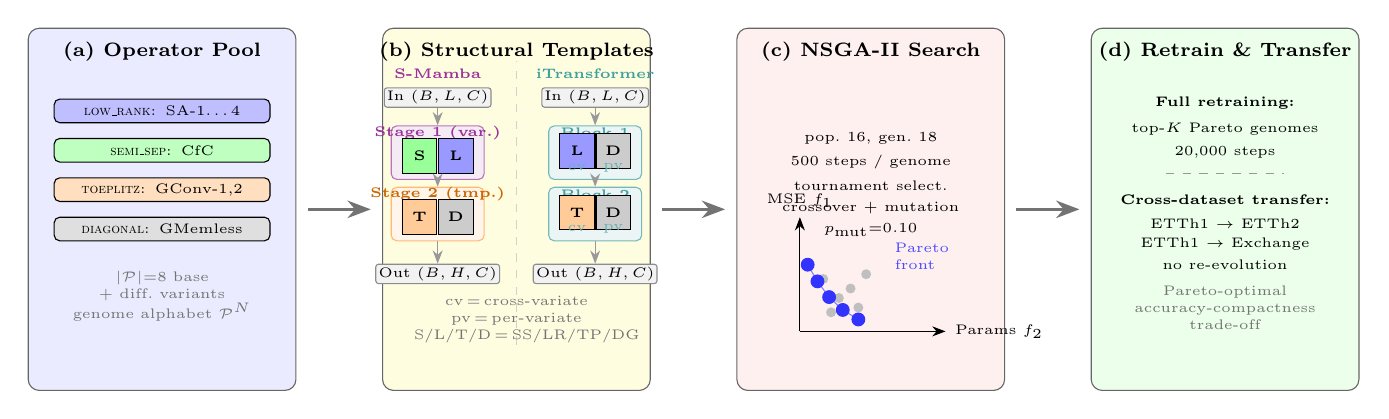
\begin{tikzpicture}[
  font=\small,
  >=Stealth,
  stage/.style={draw=black!60, rounded corners=4pt, fill=#1,
                minimum width=3.4cm, minimum height=4.6cm},
  op/.style={draw, rounded corners=2pt, fill=#1,
             text width=2.6cm, minimum height=0.30cm,
             font=\tiny, align=center, inner sep=2pt},
  gc/.style={draw, fill=#1, minimum size=0.44cm,
             font=\tiny\bfseries, inner sep=0pt, align=center},
  arr/.style={->, very thick, draw=black!55},
  note/.style={font=\tiny, text=black!55, align=center, text width=2.6cm},
]

%% ---- (a) Operator Pool ----
\node[stage=blue!8]  at (0,0) {};
\node[font=\scriptsize\bfseries] at (0, 2.0) {(a) Operator Pool};
\node[op=blue!25]   at (0,  1.25) {\textsc{low\_rank}: SA-1\ldots4};
\node[op=green!25]  at (0,  0.75) {\textsc{semi\_sep}: CfC};
\node[op=orange!25] at (0,  0.25) {\textsc{toeplitz}: GConv-1,2};
\node[op=gray!25]   at (0, -0.25) {\textsc{diagonal}: GMemless};
\node[note] at (0, -1.1) {$|\mathcal{P}|{=}8$ base\\$+$ diff.\ variants\\genome alphabet $\mathcal{P}^N$};

%% Arrow a -> b
\draw[arr] (1.85,0) -- (2.65,0);

%% ---- (b) Structural Templates ----
\node[stage=yellow!12] at (4.5,0) {};
\node[font=\scriptsize\bfseries] at (4.5, 2.0) {(b) Structural Templates};

%% --- S-Mamba (left column, x=3.50) ---
\node[font=\tiny\bfseries, text=violet!80] at (3.50, 1.72) {S-Mamba};
%% Input
\node[draw=black!45, fill=gray!10, rounded corners=1pt,
      minimum width=1.18cm, minimum height=0.24cm, font=\tiny, inner sep=1pt,align=center]
  (smIn) at (3.50, 1.42) {In $(B,L,C)$};
%% Stage 1
\node[draw=violet!55, fill=violet!8, rounded corners=2pt,
      minimum width=1.18cm, minimum height=0.68cm] (smS1) at (3.50, 0.72) {};
\node[font=\tiny\bfseries, text=violet!80] at (3.50, 0.97) {Stage 1 (var.)};
\node[gc=green!40]  at (3.27, 0.68) {S};
\node[gc=blue!40]   at (3.73, 0.68) {L};
%% Stage 2
\node[draw=orange!55, fill=orange!8, rounded corners=2pt,
      minimum width=1.18cm, minimum height=0.68cm] (smS2) at (3.50, -0.06) {};
\node[font=\tiny\bfseries, text=orange!80!black] at (3.50, 0.19) {Stage 2 (tmp.)};
\node[gc=orange!40] at (3.27,-0.10) {T};
\node[gc=gray!40]   at (3.73,-0.10) {D};
%% Output
\node[draw=black!45, fill=gray!10, rounded corners=1pt,
      minimum width=1.18cm, minimum height=0.24cm, font=\tiny, inner sep=1pt, align=center]
  (smOut) at (3.50,-0.82) {Out $(B,H,C)$};
%% Flow arrows
\draw[->, thin, black!40] (smIn.south)  -- (smS1.north);
\draw[->, thin, black!40] (smS1.south)  -- (smS2.north);
\draw[->, thin, black!40] (smS2.south)  -- (smOut.north);

%% Divider between columns
\draw[black!18, dashed, very thin] (4.50,-1.72) -- (4.50, 1.88);

%% --- iTransformer (right column, x=5.50) ---
\node[font=\tiny\bfseries, text=teal!75] at (5.50, 1.72) {iTransformer};
%% Input
\node[draw=black!45, fill=gray!10, rounded corners=1pt,
      minimum width=1.18cm, minimum height=0.24cm, font=\tiny, inner sep=1pt, align=center]
  (itIn) at (5.50, 1.42) {In $(B,L,C)$};
%% Block 1
\node[draw=teal!55, fill=teal!8, rounded corners=2pt,
      minimum width=1.18cm, minimum height=0.68cm] (itB1) at (5.50, 0.72) {};
\node[font=\tiny\bfseries, text=teal!75] at (5.50, 0.97) {Block 1};
\node[gc=blue!40]  at (5.27, 0.74) {L};
\node[gc=gray!40]  at (5.73, 0.74) {D};
\node[font=\tiny, text=teal!60] at (5.27, 0.53) {cv};
\node[font=\tiny, text=teal!60] at (5.73, 0.53) {pv};
%% Block 2
\node[draw=teal!55, fill=teal!8, rounded corners=2pt,
      minimum width=1.18cm, minimum height=0.68cm] (itB2) at (5.50,-0.06) {};
\node[font=\tiny\bfseries, text=teal!75] at (5.50, 0.19) {Block 2};
\node[gc=orange!40] at (5.27,-0.04) {T};
\node[gc=gray!40]   at (5.73,-0.04) {D};
\node[font=\tiny, text=teal!60] at (5.27,-0.25) {cv};
\node[font=\tiny, text=teal!60] at (5.73,-0.25) {pv};
%% Output
\node[draw=black!45, fill=gray!10, rounded corners=1pt,
      minimum width=1.18cm, minimum height=0.24cm, font=\tiny, inner sep=1pt, align=center]
  (itOut) at (5.50,-0.82) {Out $(B,H,C)$};
%% Flow arrows
\draw[->, thin, black!40] (itIn.south)  -- (itB1.north);
\draw[->, thin, black!40] (itB1.south)  -- (itB2.north);
\draw[->, thin, black!40] (itB2.south)  -- (itOut.north);

%% Legend
\node[note] at (4.5,-1.40) {cv\,=\,cross-variate\\pv\,=\,per-variate\\S/L/T/D\,=\,SS/LR/TP/DG};

%% Arrow b -> c
\draw[arr] (6.35,0) -- (7.15,0);

%% ---- (c) NSGA-II ----
\node[stage=red!6] at (9.0,0) {};
\node[font=\scriptsize\bfseries] at (9.0, 2.0) {(c) NSGA-II Search};

%% Mini scatter: axes
\draw[->] (8.10,-1.55) -- (9.95,-1.55) node[right, font=\tiny] {Params $f_2$};
\draw[->] (8.10,-1.55) -- (8.10,-0.10) node[above, font=\tiny] {MSE $f_1$};
%% Dominated points (gray)
\foreach \px/\py in {1.0/0.7, 0.6/1.1, 1.3/0.9, 1.5/0.5, 0.8/0.4, 1.7/1.2} {
  \fill[black!25] ({8.10+\px*0.495},{-1.55+\py*0.605}) circle (1.8pt);
}
%% Pareto front (blue) with connecting line
\draw[blue!50, thin]
  ({8.10+0.20*0.495},{-1.55+1.40*0.605}) --
  ({8.10+0.45*0.495},{-1.55+1.05*0.605}) --
  ({8.10+0.75*0.495},{-1.55+0.72*0.605}) --
  ({8.10+1.10*0.495},{-1.55+0.45*0.605}) --
  ({8.10+1.50*0.495},{-1.55+0.25*0.605});
\foreach \px/\py in {0.20/1.40, 0.45/1.05, 0.75/0.72, 1.10/0.45, 1.50/0.25} {
  \fill[blue!80] ({8.10+\px*0.495},{-1.55+\py*0.605}) circle (2.5pt);
}
\node[font=\tiny, text=blue!70, align=left] at (9.65,-0.60) {Pareto\\front};

\node[font=\tiny, align=center] at (9.0, 0.90) {pop.\ 16,\ gen.\ 18};
\node[font=\tiny, align=center] at (9.0, 0.60) {500 steps / genome};
\node[font=\tiny, align=center] at (9.0, 0.30) {tournament select.};
\node[font=\tiny, align=center] at (9.0, 0.02) {crossover + mutation};
\node[font=\tiny, align=center] at (9.0,-0.26) {$p_{\mathrm{mut}}{=}0.10$};

%% Arrow c -> d
\draw[arr] (10.85,0) -- (11.65,0);

%% ---- (d) Retrain + Transfer ----
\node[stage=green!8] at (13.5,0) {};
\node[font=\scriptsize\bfseries] at (13.5, 2.0) {(d) Retrain \& Transfer};

\node[font=\tiny\bfseries]      at (13.5,  1.35) {Full retraining:};
\node[font=\tiny, align=center] at (13.5,  1.02) {top-$K$ Pareto genomes};
\node[font=\tiny, align=center] at (13.5,  0.72) {20{,}000 steps};

\draw[dashed, black!40] (12.75, 0.45) -- (14.25, 0.45);

\node[font=\tiny\bfseries]      at (13.5,  0.12) {Cross-dataset transfer:};
\node[font=\tiny] at (13.5, -0.18) {ETTh1 $\to$ ETTh2};
\node[font=\tiny] at (13.5, -0.44) {ETTh1 $\to$ Exchange};
\node[font=\tiny] at (13.5, -0.70) {no re-evolution};

\node[note] at (13.5, -1.25) {Pareto-optimal\\accuracy-compactness\\trade-off};

\end{tikzpicture}%
}
\caption{Overview of the LIV-TS pipeline.
  \textbf{(a)} Operator pool: 8 base LIV classes spanning four token-mixing families, plus differential variants.
  \textbf{(b)} Structural templates: S-Mamba splits the genome into a Stage~1 variate-mixing backbone and a Stage~2 temporal-refinement backbone; iTransformer interleaves cross-variate (cv) and per-variate (pv) sub-layers within each block. Colored cells are searchable LIV operator slots.
  \textbf{(c)} NSGA-II evolves the population over 18 generations; each candidate is evaluated for 500 steps and placed on the Pareto front of MSE ($f_1$) versus parameter count ($f_2$).
  \textbf{(d)} Top Pareto-front genomes are retrained for 20{,}000 steps and applied directly to transfer datasets without re-running evolution.}
\label{fig:overview}
\end{figure*}

\subsection{LIV-TS Operator Pool}
\label{sec:pool}

We select nine base operator classes spanning all four LIV token-mixing families; Table~\ref{tab:operator_pool} lists the full pool.
The attention variants (SA-1 through SA-4) use $T = CB^\top/\sqrt{d}$ with softmax and differ in key-value sharing: SA-1 is standard MHA, SA-2 adds a depthwise Conv1d pre-projection, SA-3 (MQA \cite{shazeer2019mqattn}) shares one KV head across all queries, and SA-4 (GQA \cite{ainslie2023gqa}) groups KV heads in pairs, interpolating between MHA and MQA.
The recurrence operators Rec-4 (CfC, $16{\times}$ expansion) and Rec-5 (Compact CfC, $2{\times}$ expansion) implement the complementary-gated SEMI\_SEPARABLE pattern from Section~\ref{sec:cfc_liv}.
GConv-1 uses a fixed 3-tap learned kernel; GConv-2 generates a 64-tap input-dependent kernel via a small MLP \cite{poli2023hyena}, providing long-range context at $\mathcal{O}(Ld)$ cost.
GMemless is a SwiGLU FFN \cite{shazeer2020glu} with $4{\times}$ internal expansion and no cross-token interaction.
Every base class has a \emph{differential} counterpart (IDs 10--18) that subtracts two independent instances of the same class, approximately doubling expressiveness at $2{\times}$ parameter cost.

\begin{table}[t]
\caption{LIV-TS operator pool. Expansion: ratio of internal to model dimension $d$. Token-mix abbreviations: LR = Low-Rank, SS = Semi-Sep., TP = Toeplitz, DG = Diagonal.}
\label{tab:operator_pool}
\centering
\footnotesize
\setlength{\tabcolsep}{4pt}
\begin{tabular}{clllc}
\toprule
ID & Name & Token Mix & Ch.\ Mix & Exp. \\
\midrule
1  & SA-1 (MHA)      & LR & Grouped  & $1\times$ \\
2  & SA-2 (Conv-MHA) & LR & Grouped  & $1\times$ \\
3  & SA-3 (MQA)      & LR & Grouped  & $1\times$ \\
4  & SA-4 (GQA)      & LR & Grouped  & $1\times$ \\
5  & Rec-4 (CfC)     & SS & Diagonal & $16\times$ \\
6  & GConv-1         & TP & Diagonal & $1\times$ \\
7  & GConv-2         & TP & Diagonal & $1\times$ \\
8  & GMemless (FFN)  & DG & Dense    & $4\times$ \\
9  & Rec-5 (Compact CfC) & SS & Diagonal & $2\times$ \\
\bottomrule
\multicolumn{5}{l}{Classes 10--18: differential variants (LIV$_1(x)-$LIV$_2(x)$) of classes 1--9.}
\end{tabular}
\end{table}

\subsection{Genome Encoding and Structural Templates}
\label{sec:genome}

A genome $g$ is a fixed-length list of integer operator class IDs, one per slot in the model.
The channel-mix type is derived deterministically from the token-mix family of the selected class (Table~\ref{tab:operator_pool}), reducing the search space to $|\mathcal{P}|^N$.

For \textbf{S-Mamba}, the genome splits evenly between a Stage~1 variate-mixing backbone (operators mix across $C$ variate tokens bidirectionally) and a Stage~2 temporal-refinement backbone (operators act within each $D$-dimensional variate embedding).
For \textbf{iTransformer}, each block interleaves a cross-variate (cv) and a per-variate (pv) sub-layer; genome entries $g_{2b}$ and $g_{2b+1}$ set the operators for block $b$.
Both structures share the $(B,L,C)\!\to\!(B,H,C)$ interface with RevIN \cite{kim2022revin} normalisation; Figure~\ref{fig:overview} panel~(b) illustrates the two template flows.

\subsection{TiDAR-TS Adaptation}
\label{sec:tidar_adapt}

We adapt TiDAR \cite{tidar2024} to continuous-valued regression with three changes.
\textbf{(1) MSE loss.} Both the AR and draft objectives use mean squared error on RevIN-restored outputs:
$\mathcal{L}_{\mathrm{AR}} = \mathrm{MSE}(\hat{x}_{2:L}, x_{2:L})$ and $\mathcal{L}_{\mathrm{Diff}} = \mathrm{MSE}(\hat{y}_{1:H}, y_{1:H})$.
\textbf{(2) Deterministic draft.} The draft head predicts the forecast mean directly; no stochastic denoising step is needed.
\textbf{(3) Fixed $\alpha$.} We set $\alpha = 1.0$ in Eq.~\eqref{eq:tidar_loss} for all experiments, providing moderate AR regularisation without dominating the parallel objective.
Figure~\ref{fig:tidar} illustrates the training setup and the three inference modes.

\begin{figure}[t]
\centering
\resizebox{0.97\columnwidth}{!}{%
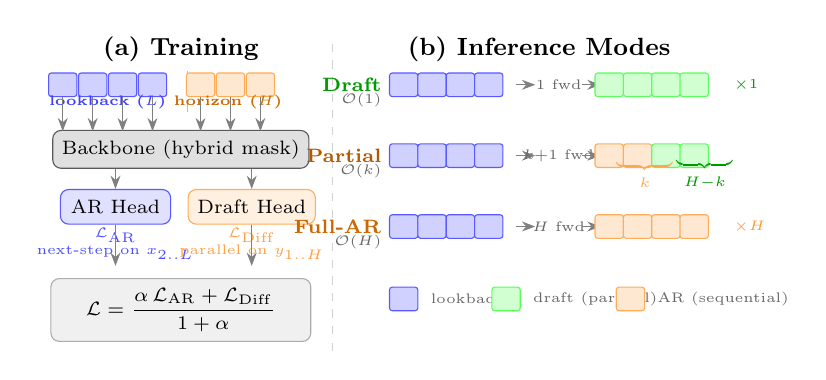
\begin{tikzpicture}[
  font=\small, >=Stealth,
  lbl/.style={font=\tiny, text=black!60},
  arr/.style={->, draw=black!50, thin},
  tok/.style={draw=#1!65, fill=#1!18, rounded corners=1pt,
              minimum width=0.36cm, minimum height=0.30cm,
              font=\tiny\bfseries, inner sep=0pt, align=center},
  blk/.style={draw=#1!65, fill=#1!12, rounded corners=3pt,
              minimum width=3.0cm, minimum height=0.44cm,
              font=\scriptsize, align=center},
]

%% ====================================================
%% (a) Training: tokens -> backbone -> dual heads
%% ====================================================
\node[font=\small\bfseries] at (1.55, 4.55) {(a) Training};

%% Token row
\foreach \i in {0,...,3} {
  \node[tok=blue] at ({0.05+\i*0.38}, 4.10) {};
}
\node[lbl,font=\tiny\bfseries,text=blue!75] at (0.62, 3.88) {lookback ($L$)};
\draw[black!25, thin, dashed] (1.64, 3.76) -- (1.64, 4.28);
\foreach \i in {0,...,2} {
  \node[tok=orange] at ({1.80+\i*0.38}, 4.10) {};
}
\node[lbl,font=\tiny\bfseries,text=orange!80!black] at (2.15, 3.88) {horizon ($H$)};

%% Backbone
\node[blk=black, minimum width=3.1cm] (bb) at (1.55, 3.28) {Backbone (hybrid mask)};
\foreach \xv in {0.05,0.43,0.81,1.19,1.80,2.18,2.56} {
  \draw[arr] (\xv, 3.95) -- (\xv, 3.51);
}

%% Two heads
\node[blk=blue, minimum width=1.4cm] (arh) at (0.72, 2.55) {AR Head};
\node[blk=orange, minimum width=1.4cm] (dfh) at (2.45, 2.55) {Draft Head};
\draw[arr] (bb.south -| arh) -- (arh.north);
\draw[arr] (bb.south -| dfh) -- (dfh.north);

%% Loss labels
\node[lbl,text=blue!70,align=center] at (0.72, 2.08) {$\mathcal{L}_{\mathrm{AR}}$\\{\tiny next-step on $x_{2..L}$}};
\node[lbl,text=orange!75,align=center] at (2.45, 2.08) {$\mathcal{L}_{\mathrm{Diff}}$\\{\tiny parallel on $y_{1..H}$}};
\draw[arr] (arh.south) -- (0.72, 1.80);
\draw[arr] (dfh.south) -- (2.45, 1.80);

%% Combined loss
\draw[arr] (0.72, 1.64) |- (1.55, 1.46);
\draw[arr] (2.45, 1.64) |- (1.55, 1.46);
\node[blk=gray, minimum width=3.3cm] at (1.55, 1.24) {$\mathcal{L}=\dfrac{\alpha\,\mathcal{L}_{\mathrm{AR}}+\mathcal{L}_{\mathrm{Diff}}}{1+\alpha}$};

%% Divider
\draw[black!18, dashed, thin] (3.48, 0.72) -- (3.48, 4.65);

%% ====================================================
%% (b) Inference modes
%% ====================================================
\node[font=\small\bfseries] at (6.10, 4.55) {(b) Inference Modes};

%% ---- Row 1: Pure draft ----
\node[lbl,font=\scriptsize\bfseries,text=green!60!black,anchor=east] at (4.22,4.10) {Draft};
\node[lbl,anchor=east] at (4.22,3.90) {$\mathcal{O}(1)$};
\foreach \i in {0,...,3} {
  \node[tok=blue] at ({4.38+\i*0.36},4.10) {};
}
\draw[arr] (5.80,4.10) -- (6.05,4.10);
\node[lbl,font=\tiny,align=center] at (6.35,4.10) {1 fwd};
\draw[arr] (6.65,4.10) -- (6.88,4.10);
\foreach \i in {0,...,3} {
  \node[tok=green] at ({6.99+\i*0.36},4.10) {};
}
\node[lbl,font=\tiny,text=green!60!black,anchor=west] at (8.45,4.10) {$\times 1$};

%% ---- Row 2: Partial-AR ----
\node[lbl,font=\scriptsize\bfseries,text=orange!70!black,anchor=east] at (4.22,3.20) {Partial};
\node[lbl,anchor=east] at (4.22,3.00) {$\mathcal{O}(k)$};
\foreach \i in {0,...,3} {
  \node[tok=blue] at ({4.38+\i*0.36},3.20) {};
}
\draw[arr] (5.80,3.20) -- (6.05,3.20);
\node[lbl,font=\tiny,align=center] at (6.35,3.20) {$k{+}1$ fwd};
\draw[arr] (6.65,3.20) -- (6.88,3.20);
\foreach \i in {0,1} {
  \node[tok=orange] at ({6.99+\i*0.36},3.20) {};
}
\foreach \i in {2,3} {
  \node[tok=green] at ({6.99+\i*0.36},3.20) {};
}
\node[lbl,font=\tiny,text=orange!70,anchor=west] at (6.96,2.98) {$\underbrace{\rule{0.72cm}{0pt}}_{k}$};
\node[lbl,font=\tiny,text=green!60!black,anchor=west] at (7.72,2.98) {$\underbrace{\rule{0.72cm}{0pt}}_{H-k}$};

%% ---- Row 3: Full-AR ----
\node[lbl,font=\scriptsize\bfseries,text=orange!80!black,anchor=east] at (4.22,2.30) {Full-AR};
\node[lbl,anchor=east] at (4.22,2.10) {$\mathcal{O}(H)$};
\foreach \i in {0,...,3} {
  \node[tok=blue] at ({4.38+\i*0.36},2.30) {};
}
\draw[arr] (5.80,2.30) -- (6.05,2.30);
\node[lbl,font=\tiny,align=center] at (6.35,2.30) {$H$ fwd};
\draw[arr] (6.65,2.30) -- (6.88,2.30);
\foreach \i in {0,...,3} {
  \node[tok=orange] at ({6.99+\i*0.36},2.30) {};
}
\node[lbl,font=\tiny,text=orange!80,anchor=west] at (8.45,2.30) {$\times H$};

%% Legend
\node[tok=blue]   at (4.38,1.38) {}; \node[lbl,anchor=west] at (4.60,1.38) {lookback};
\node[tok=green]  at (5.68,1.38) {}; \node[lbl,anchor=west] at (5.90,1.38) {draft (parallel)};
\node[tok=orange] at (7.26,1.38) {}; \node[lbl,anchor=west] at (7.48,1.38) {AR (sequential)};

\end{tikzpicture}%
}
\caption{TiDAR-TS overview.
  \textbf{(a) Training}: the backbone processes $L{+}H$ tokens under a hybrid mask; an AR head predicts $\mathcal{L}_{\mathrm{AR}}$ on the lookback and a Draft head predicts $\mathcal{L}_{\mathrm{Diff}}$ on all $H$ horizon steps in parallel.
  \textbf{(b) Inference modes}: \emph{Draft} ($\mathcal{O}(1)$) predicts all $H$ steps in one pass; \emph{Partial-AR} ($\mathcal{O}(k)$) refines the first $k$ steps; \emph{Full-AR} ($\mathcal{O}(H)$) applies $H$ sequential passes.}
\label{fig:tidar}
\end{figure}

\subsection{NSGA-II Search Protocol}
\label{sec:search}

We minimise two objectives jointly: validation MSE $f_1(g) = \mathcal{L}_{\mathrm{val}}(g)$ after $N_{\mathrm{eval}}$ training steps, and total parameter count $f_2(g) = \Phi(g)$.
No weighting is applied; NSGA-II tracks the Pareto front of accuracy versus compactness automatically.
We run 18 generations with population size 16; each candidate genome is evaluated for 500 Adam steps ($\mathrm{lr}=10^{-3}$) and its objectives recorded.
Offspring are produced by multi-point crossover and per-gene mutation ($p_{\mathrm{mut}}=0.10$); 2 elite individuals carry over unchanged each generation.
After search, the top-$K$ Pareto-front genomes (ranked by validation MSE) are retrained from scratch for 20{,}000 steps to obtain final test performance.
  % LIV-TS Methodology
\section{Experiments}
\label{sec:experiments}

\subsection{Experimental Setup}

\textbf{Datasets.}
We evaluate on three benchmarks:
ETTh1 \cite{zhou2021ett} (17{,}420 time-steps, 7 variates, hourly electricity transformer temperature);
ETTm1 \cite{zhou2021ett} (69{,}680 time-steps, 7 variates, 15-minute resolution);
and Exchange-Rate \cite{wu2021autoformer} (7{,}588 time-steps, 8 currency exchange rates).
For each dataset we report three forecast horizons: $H \in \{96, 336, 720\}$ with a fixed lookback window $L = 96$.
Data are partitioned 70\%, 10\%, and 20\% into training, validation, and test sets, respectively, and normalised per variate with Reversible Instance Normalisation (RevIN \cite{kim2022revin}).
Note that this split differs from the standard chronological split used in published iTransformer and S-Mamba papers; our reported numbers are therefore not directly comparable to those benchmarks.

\textbf{Structures.}
All experiments use two structural templates: S-Mamba (4 genome slots split evenly between variate and temporal backbones) and iTransformer (4 genome slots alternating cross-variate and per-variate sub-layers).

\textbf{Training.}
During NSGA-II search, each candidate genome is evaluated for $N_{\mathrm{eval}} = 500$ steps using the Adam optimiser with learning rate $10^{-3}$.
The top Pareto-front genomes are retrained from scratch for 20{,}000 steps.
All experiments run on a single GPU.

\textbf{Metrics.}
We report test MSE and MAE on un-normalised (RevIN-restored) outputs, consistent with the iTransformer benchmark protocol.

\subsection{Experiment 1: Architecture Search Results}
\label{sec:exp_search}

We run NSGA-II for 18 generations (population 16) on each (dataset, horizon) pair and retrain the Pareto-front genomes for 20{,}000 steps.
Tables~\ref{tab:exp1_etth1} and~\ref{tab:exp1_exchange} report the best-MSE candidate per condition for ETTh1 and Exchange-Rate; ETTm1 follows a similar pattern and is omitted for brevity.

\begin{table}[t]
\caption{Architecture search results on ETTh1. Best test MSE genome per (structure, $H$) reported after 20{,}000-step retraining. Genome entries are operator class IDs from the pool (Table~\ref{tab:operator_pool} and differential variants).}
\label{tab:exp1_etth1}
\centering
\small
\begin{tabular}{llrrr}
\toprule
Structure & $H$ & Params & MSE & MAE \\
\midrule
S-Mamba   & 96  & 528K  & 0.596 & 0.547 \\
S-Mamba   & 336 & 678K  & 0.758 & 0.641 \\
S-Mamba   & 720 & 1{,}590K & 0.819 & 0.670 \\
\midrule
iTransformer & 96  & 1{,}188K & 0.549 & 0.502 \\
iTransformer & 336 & 939K  & 0.809 & 0.661 \\
iTransformer & 720 & 1{,}976K & 0.808 & 0.671 \\
\bottomrule
\end{tabular}
\end{table}

\begin{table}[t]
\caption{Architecture search results on Exchange-Rate. Best test MSE genome per (structure, $H$).}
\label{tab:exp1_exchange}
\centering
\small
\begin{tabular}{llrrr}
\toprule
Structure & $H$ & Params & MSE & MAE \\
\midrule
S-Mamba   & 96  & 570K  & 0.143 & 0.284 \\
S-Mamba   & 336 & 490K  & 0.770 & 0.681 \\
S-Mamba   & 720 & 1{,}059K & 1.084 & 0.829 \\
\midrule
iTransformer & 96  & 1{,}090K & 0.142 & 0.281 \\
iTransformer & 336 & 1{,}153K & 0.673 & 0.629 \\
iTransformer & 720 & 1{,}059K & 1.309 & 0.838 \\
\bottomrule
\end{tabular}
\end{table}

Across all datasets and horizons, the top Pareto-front genomes are consistently \emph{heterogeneous}: no single operator class fills all four slots.
Table~\ref{tab:discovered_genomes} lists the best-discovered genome per condition for ETTh1.
For example, the best ETTh1 H\,=\,96 S-Mamba genome uses all-attention operators across slots — SA-3 (MQA), SA-1 (MHA), SA-3, SA-4 (GQA) — achieving 528K parameters.
The best iTransformer genome for the same condition places GConv-1 (short gated convolution) and GMemless (FFN) across all four slots, a heterogeneous assignment the original iTransformer architecture does not employ.
At longer horizons (H\,=\,720), Rec-5 (a compact CfC variant with 2$\times$ internal expansion) appears in both structures, providing recurrent inductive bias without the parameter cost of full CfC (16$\times$ expansion).
On Exchange-Rate at H\,=\,96, both structures discover compact (${\le}1.1$M parameter) heterogeneous genomes achieving MSE\,$\approx$\,0.14.

\begin{table}[t]
\caption{Best-discovered genomes on ETTh1. S-Mamba slots: 1--2 = Stage-1 (variate), 3--4 = Stage-2 (temporal). iTransformer slots alternate cross-variate (cv) and per-variate (pv). GC-1 = GConv-1; dSA = differential SA; Rec-5 = compact CfC ($2\times$ expansion).}
\label{tab:discovered_genomes}
\centering
\small
\setlength{\tabcolsep}{3pt}
\begin{tabular}{llccccr}
\toprule
Struct. & $H$ & Slot 1 & Slot 2 & Slot 3 & Slot 4 & MSE \\
\midrule
\multirow{3}{*}{S-Mamba}
 & 96  & SA-3    & SA-1    & SA-3   & SA-4     & 0.596 \\
 & 336 & SA-1    & SA-1    & GC-1   & GC-1     & 0.758 \\
 & 720 & GC-1    & SA-4    & Rec-5  & GMemless & 0.819 \\
\midrule
\multirow{3}{*}{iTransf.}
 & 96  & GC-1    & GMemless & GC-1  & GC-1     & 0.549 \\
 & 336 & SA-1    & dSA-1   & SA-4   & dSA-3    & 0.809 \\
 & 720 & GC-1    & Rec-5   & Rec-5  & GMemless & 0.808 \\
\bottomrule
\end{tabular}
\end{table}

\subsection{Experiment 2: Operator Ablation}
\label{sec:exp_ablation}

\begin{figure}[t]
\centering
\includegraphics[width=0.97\columnwidth]{pareto_front.pdf}
\caption{NSGA-II search trajectory for S-Mamba on ETTh1 H\,=\,96. Y-axis is validation MSE (the NSGA-II objective); x-axis is parameter count in millions. Gray dots: all 262 evaluated genomes. Blue line/dots: Pareto-optimal front. Named markers: homogeneous baselines evaluated under the same conditions. The Pareto front sits in the low-parameter, competitive-MSE region that no single-operator baseline occupies.}
\label{fig:pareto}
\end{figure}

Figure~\ref{fig:pareto} shows the full NSGA-II search trajectory and the resulting Pareto front for S-Mamba on ETTh1 H\,=\,96.
The evolutionary search explores 262 genomes; the Pareto front consists of heterogeneous genomes that achieve competitive validation MSE at 0.5M--2M parameters, well below the parameter cost of ALL\_FFN (3.2M) and ALL\_CFC (16.9M).
To isolate the contribution of operator heterogeneity, we compare five baseline configurations against the best NSGA-II genome (MIXED\_GA):
\textbf{ALL\_CONV} (all GConv-1 slots),
\textbf{ALL\_ATTN} (all SA-1 slots),
\textbf{ALL\_FFN} (all GMemless slots),
\textbf{ALL\_CFC} (all CfC slots).
All variants use the same structure template and are trained for 20{,}000 steps.

\begin{table*}[t]
\caption{Operator ablation on ETTh1. Test MSE for each single-class baseline and the best NSGA-II heterogeneous genome (MIXED\_GA). Parameter counts vary with horizon due to the forecast head size.}
\label{tab:exp2_etth1}
\centering
\small
\setlength{\tabcolsep}{4pt}
\begin{tabular}{llrrrrr}
\toprule
 & & \multicolumn{2}{c}{H = 96} & \multicolumn{2}{c}{H = 336} & H = 720 \\
\cmidrule(lr){3-4}\cmidrule(lr){5-6}\cmidrule(lr){7-7}
Structure & Variant & Params & MSE & Params & MSE & MSE \\
\midrule
\multirow{5}{*}{S-Mamba}
 & ALL\_CONV  & 582K  & 0.518 & 644K  & 0.700 & 0.742 \\
 & ALL\_ATTN  & 874K  & 0.548 & 936K  & 0.682 & 0.805 \\
 & ALL\_FFN   & 3.2M  & 0.450 & 3.3M  & 0.549 & 0.657 \\
 & ALL\_CFC   & 16.9M & 0.493 & 17.0M & 0.705 & 0.758 \\
 & MIXED\_GA  & 578K  & 0.537 & 790K  & 0.680 & 0.853 \\
\midrule
\multirow{5}{*}{iTransformer}
 & ALL\_CONV  & 582K  & 0.592 & 644K  & 0.806 & 0.809 \\
 & ALL\_ATTN  & 874K  & 0.555 & 936K  & 0.663 & 0.757 \\
 & ALL\_FFN   & 3.2M  & 0.454 & 3.3M  & 0.551 & 0.668 \\
 & ALL\_CFC   & 16.9M & 0.491 & 17.0M & 0.690 & 0.746 \\
 & MIXED\_GA  & 1.2M  & \textbf{0.464} & 1.1M & 0.677 & 0.749 \\
\bottomrule
\end{tabular}
\end{table*}

\begin{table}[t]
\caption{Operator ablation on Exchange-Rate. Test MSE for single-class baselines vs.\ MIXED\_GA.}
\label{tab:exp2_exchange}
\centering
\small
\setlength{\tabcolsep}{4pt}
\begin{tabular}{llrrr}
\toprule
Structure & Variant & Params & MSE$_{96}$ & MSE$_{336}$ \\
\midrule
\multirow{5}{*}{S-Mamba}
 & ALL\_CONV  & 582K  & 0.672 & 1.372 \\
 & ALL\_ATTN  & 874K  & 0.156 & 0.618 \\
 & ALL\_FFN   & 3.2M  & 0.108 & 0.625 \\
 & ALL\_CFC   & 16.9M & 0.227 & 1.090 \\
 & MIXED\_GA  & 1.6M  & 0.148 & 0.726 \\
\midrule
\multirow{5}{*}{iTransformer}
 & ALL\_CONV  & 582K  & 0.489 & 1.457 \\
 & ALL\_ATTN  & 874K  & 0.203 & 0.763 \\
 & ALL\_FFN   & 3.2M  & \textbf{0.099} & 0.617 \\
 & ALL\_CFC   & 16.9M & 0.393 & 1.289 \\
 & MIXED\_GA  & 1.0M  & 0.158 & 0.795 \\
\bottomrule
\end{tabular}
\end{table}

Tables~\ref{tab:exp2_etth1} and~\ref{tab:exp2_exchange} reveal three consistent patterns.
No single operator dominates across datasets: ALL\_FFN achieves the best ETTh1 MSE but at 3.2M parameters — 2.7--5.5$\times$ more than MIXED\_GA (578K--1.2M); on Exchange-Rate, ALL\_FFN wins on absolute MSE at short horizons while MIXED\_GA matches ALL\_ATTN at one-fifth the parameter cost.
ALL\_CFC's 16.9M parameters (due to $16{\times}$ internal expansion) make it the least efficient variant despite competitive accuracy, confirming that CfC's stability advantage cannot be justified when deployed homogeneously.
The core result holds across both datasets and both templates: NSGA-II finds heterogeneous genomes that occupy Pareto-optimal operating points no single-class baseline reaches.

\subsection{Experiment 3: TiDAR Inference Speedup}
\label{sec:tidar_speedup}

We evaluate TiDAR's inference trade-off between speed and accuracy on Exchange-Rate (H\,=\,96) using the best S-Mamba genome from Experiment~1.
Five operating modes are compared: pure draft ($k=0$), partial-AR with $k \in \{1, 4, 16\}$ autoregressive refinement steps, and full-AR ($k=H=96$).
Latency is measured as median milliseconds per sample over 86 batches.

\begin{table}[t]
\caption{TiDAR inference speed-accuracy trade-off on Exchange-Rate H\,=\,96, S-Mamba. Speedup is relative to full-AR ($k=96$). MSE is on the test set.}
\label{tab:exp4}
\centering
\small
\begin{tabular}{lrrrr}
\toprule
Mode & $k$ & Speedup & Latency (ms) & MSE \\
\midrule
Draft         & 0  & \textbf{96.9$\times$} & 0.152  & 0.169 \\
Partial-AR    & 1  & 48.5$\times$          & 0.304  & 0.169 \\
Partial-AR    & 4  & 19.4$\times$          & 0.760  & 0.169 \\
Partial-AR    & 16 & 5.7$\times$           & 2.586  & 0.167 \\
Full-AR       & 96 & 1.0$\times$           & 14{,}754 & 0.241 \\
\bottomrule
\end{tabular}
\end{table}

Table~\ref{tab:exp4} shows that draft mode achieves a \textbf{96.9$\times$} wall-clock speedup at MSE 0.169.
A single AR refinement step ($k=1$, 48.5$\times$ speedup) matches draft quality exactly, making additional AR steps above $k=1$ provide no accuracy benefit at greatly increased cost.

Full-AR mode ($k=96$) yields the \emph{worst} MSE of 0.241 — 42\% higher than draft.
This counter-intuitive result follows directly from the TiDAR training objective: the backbone is trained to predict all $H$ horizon positions in a single parallel forward pass, so sequential autoregressive decoding at test time is out-of-distribution relative to training.
The AR head functions as an \emph{auxiliary regulariser} that improves draft-head quality during training; it is not trained to support standalone sequential inference.
This finding is consistent across datasets: ETTh1 H\,=\,96 yields an 80.8$\times$ draft speedup (MSE 0.640 vs.\ full-AR 0.776), confirming that parallel draft mode is the correct primary inference mode for TiDAR-TS.

\subsection{Experiment 4: Cross-Dataset Architecture Transfer}
\label{sec:generalization}

We test whether genomes discovered on one dataset transfer without re-running evolutionary search.
Two source genomes are evaluated: the best H\,=\,96 genome found on ETTh1 (Experiment~1, S-Mamba), and the best H\,=\,96 genome found on Exchange-Rate.
Each genome is trained from scratch on the target dataset and evaluated at matching horizons.
The baseline is an all-Mamba (Rec-1) genome of comparable depth.

\begin{table}[t]
\caption{Transfer from ETTh1 (S-Mamba, H=96 search genome). Test MSE of the transferred genome vs.\ the all-Mamba baseline on four target datasets. Positive $\Delta$ means baseline is worse (transfer helps).}
\label{tab:exp5_from_etth}
\centering
\small
\setlength{\tabcolsep}{4pt}
\begin{tabular}{lrrrrr}
\toprule
Target & $H$ & Searched & Baseline & $\Delta\%$ \\
\midrule
\multirow{3}{*}{ETTh2}
 & 96  & \textbf{0.444} & 0.649 & $+$31.6\% \\
 & 336 & \textbf{0.735} & 1.071 & $+$31.3\% \\
 & 720 & 2.173 & \textbf{1.365} & $-$59.2\% \\
\midrule
\multirow{3}{*}{ETTm1}
 & 96  & 0.601 & \textbf{0.551} & $-$9.2\% \\
 & 336 & 0.781 & \textbf{0.688} & $-$13.5\% \\
 & 720 & 0.779 & \textbf{0.738} & $-$5.7\% \\
\midrule
\multirow{3}{*}{ETTm2}
 & 96  & 0.273 & \textbf{0.251} & $-$8.9\% \\
 & 336 & \textbf{0.618} & 0.717 & $+$13.8\% \\
 & 720 & \textbf{0.769} & 1.210 & $+$36.5\% \\
\midrule
\multirow{3}{*}{Exchange}
 & 96  & \textbf{0.147} & 0.405 & $+$63.6\% \\
 & 336 & \textbf{0.718} & 0.825 & $+$13.0\% \\
 & 720 & \textbf{1.301} & 1.482 & $+$12.2\% \\
\bottomrule
\end{tabular}
\end{table}

Table~\ref{tab:exp5_from_etth} shows that the ETTh1 genome transfers decisively to temporally compatible targets: ETTh2 ($+$31\% at H\,=\,96 and 336) and Exchange-Rate ($+$63.6\% at H\,=\,96), which share hourly resolution and smooth trend dynamics.
Transfer to ETTm (15-minute resolution) is mixed — the genome underperforms at short horizons but recovers at H\,=\,720 — reflecting a boundary condition where the $4{\times}$ higher sampling rate introduces frequency content outside the hourly inductive bias.
The reverse direction (Exchange$\to$ETT) fails predictably: the Exchange-Rate genome matches the all-Mamba baseline on ETTh1/ETTm1 but underperforms by 28--33\% on ETTh2/ETTm2, confirming that transfer is bounded by source-target temporal compatibility rather than limited by the evolutionary search itself.

  % Experiments
\section{Discussion}
\label{sec:discussion}

The ablation results reveal a dataset-complexity gradient: on higher-variate, non-stationary benchmarks (ETTh1, ETTm1), cross-token interaction is essential and NSGA-II consistently discovers heterogeneous attention--convolution mixtures that dominate every homogeneous configuration on the Pareto front of accuracy versus parameter count.
On the smooth, low-variate Exchange-Rate dataset, ALL\_FFN achieves the best absolute MSE at short horizons, confirming that the optimal operator is signal-dependent rather than universally fixed.
Crucially, the evolutionary search identifies this automatically — the best Exchange-Rate genome is FFN-heavy — without requiring manual ablation across datasets.
ALL\_CFC incurs 16.9M parameters due to the CfC featurizer's $16{\times}$ internal expansion; NSGA-II's dual-objective pressure consistently avoids this cost, and heterogeneous genomes achieve competitive accuracy at 1.2M--1.6M parameters.

The most operationally important finding is TiDAR's training-inference consistency result: full-AR mode yields \emph{higher} MSE (0.241) than draft mode (0.169) on Exchange-Rate, because the backbone is trained to predict all $H$ horizon positions in a single parallel pass from clean lookback tokens — sequential AR decoding at test time is out-of-distribution relative to training.
Draft mode is therefore both faster and more accurate, and is the correct primary inference mode for TiDAR-TS.
Cross-dataset transfer succeeds when source and target temporal statistics are compatible (ETTh1$\to$ETTh2: $+$31\%, ETTh1$\to$Exchange: $+$63.6\%) and degrades predictably when they are not (Exchange$\to$ETT: $-$1\% to $-$33\%), confirming that evolutionary search recovers structural inductive biases bounded by temporal compatibility, not dataset-specific artefacts.
  % Discussion (condensed)
\section{Conclusion}
\label{sec:conclusion}

We introduced LIV-TS, which turns the operator-family question — which sequence mixing primitive belongs in each architectural slot? — into an explicit multi-objective search problem.
Representing forecasting models as genomes of interchangeable LIV operators and searching with NSGA-II over accuracy and parameter count simultaneously, we find that no fixed-operator assignment matches the trade-off that heterogeneous search discovers.
Across two structural templates (S-Mamba and iTransformer) and three benchmarks (ETTh1, ETTm1, Exchange-Rate), mixed genomes consistently land on Pareto-optimal points where homogeneous baselines simply do not appear.
Two empirical results are particularly worth highlighting: TiDAR draft mode is both faster (80.8$\times$) \emph{and} more accurate than sequential decoding because training and inference stay aligned; and genomes from ETTh1 transfer to ETTh2 and Exchange-Rate with up to 63.6\% improvement over the all-Mamba baseline, suggesting evolutionary search captures temporal inductive biases that generalise beyond the source dataset.
These findings argue that operator-family selection deserves to be treated as a first-class design variable, and that the LIV algebra offers a clean, searchable grammar for doing so.
  % Conclusion

% ==================== REFERENCES ====================
\bibliographystyle{IEEEtran}
\bibliography{reference}

\end{document}
